\section{Spoler}

En spole er en noget der bliver brugt til mange forskellige ting, men det spolen bruges til er, at der sendes strøm igennem spolen, når strømen er blevet sendt igennem opstår der et magnetfelt om spolen. Magnetfeltet der bliver dannet omkring spolen, vil ligne det fra en magnet, men skal være af samme form så spolen. Feltet bliver meget kraftigere hvis der er jern inde i spolen. 

Hvis spolen kortsluttes mens der er strøm der løber igennem, vil spolen på bedst muligvis forsøge at opretholde strømmen, men da strømmen ikke kan løbe i en kreds kan det ikke lade sig gøre for spolen og opretholde strømmen.  Strømmen bruges i stedet i feltet, det vil sige at spændingen over spolens ender stiger voldsomt og der opstår ofte en gnist. Det er det samme der sker i tænd spolen i bilen eller i et køkken apparat eller lignende.

\begin{figure}[htbp]
	\centering
	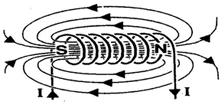
\includegraphics[width=0.5
	\textwidth]{Vildledning/Schematics/magnetfelt_omkring_en_spole.png}
	\caption{Magnetfelt omkring en spole.\cite{spoler}}
	\label{spole1}
\end{figure}

En magnet der er permanent er også en metalgering, som der ofte er jern i, magneten for derved den egenskab, at den bliver magnetisk.  Bliver en permanent magnet skubbet over til noget der er kortsluttede, det kan være en spole sker der det, at den permanente magnet vil fremkalde strøm i spolen, når der er fremkaldt en strøm vil den permanente magnet forsøge, at holde feltet ude. Det betyder at spolen forsøger, at lave poler, som vil vende modsat af den permanente magnet. Men strømen vil i løbet af meget kort tid forsvinde, hvis magneten ligger stille dette skyldes, at energien/strømen vil blive omdannet til varme inde i spolens modstand. Hvis magneten derimod bliver fjernet sker der omvendte, altså vil den påbegynde i det modsat retning, altså starte fra det felt der var inden magneten blev tilføjet. Ud fra dette kan det konkluderes, at der kun er strøm i spolen når der enten sættes et batteri til eller mag-netfeltet ændres. Hvis feltet forbliver konstant vil strømen forsvinde hurtigt og gå i nul dette skyldes også den ohmske modstand. 

En spole har ud fra dette altså ingen magnetfelt, medmindre den bliver påvirket af strøm eller man påvirker den vedhjælp af magnetisme. 

Der findes en række stoffer ved lave temperaturer disse stoffer er superledende, som også betyder, at de ingen elektrisk modstand har, når de ingen elektrisk modstand har ligger modstanden på $0 \Omega$. Der er tale om legeringer af stoffer der er sjældne, men er almindelig kendte i blandt andet bly og kviksølv. Laves der en blyring, bly ringen bliver sat ved stuetemperatur hvor der bliver sat en permanent magnet igen-nem, hvis nu det hele bliver kølet ned til det absolutte nulpunkt som ca. er $-273^\circ C$, når dette er gjort fjernes den permanente magnet, når den permanente magnet er blevet fjernet vil der ske det, som normalt sker ved induktion der vil nemlig opstå en strøm i blyringen, den strøm der opstår vil sørger for og gen-skabe det magnetfelt, som den permanente magnet havde. Der er ingen modsat hvilket også vil gøre, at strømmen vil forsætte så der haves et konstant magnetfelt, som er magen til det oprindelige magnetfelt. Magnetfeltet bliver målt i en enhed kaldet Tesla, som er opkaldt efter Nikola Tesla 1856-1943. \cite{spoler}

